\newpage

\section{Facemark} \label{section:landmarks}

\textit{Facemarks} (lub \textit{Face landmarks}) to punkty nakładane na twarz wokół interesujących obszarów - takich jak oczy, nos czy usta. Pozwalają określić położenie, rozmiar czy kształt tych obiektów. Mogą być również użyte do predykcji czy mamy zamknięte/otwarte oczy (patrz rozdz. \hyperref[section:EARsection]{\textit{\ref{section:EARsection}.EAR}}) lub czy się uśmiechamy. 

\begin{figure}[!h]
    \begin{center}
        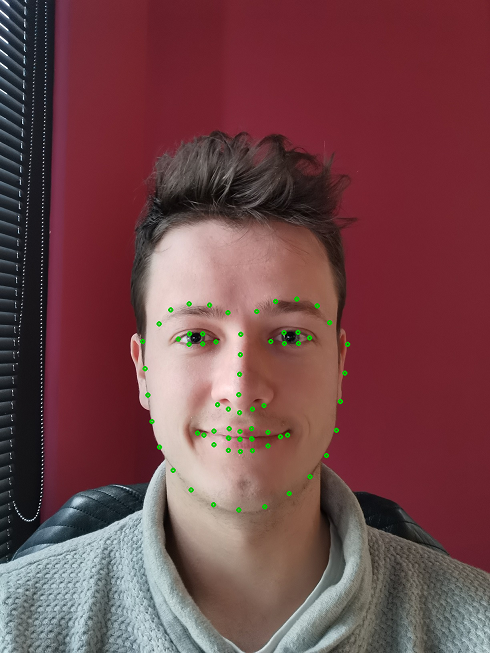
\includegraphics[scale=0.6]{img/landmark_section/landmarks_1.png}
        \caption{Przykład zdjęcia twarz z naniesionymi facemarkami}
        \label{fig:landmarks_1}
    \end{center}
\end{figure}

\subsection{Local binary features}
Metoda oparta o histogram LBF \cite{lbpFacemark}. W projekcie została użyta implementacja tego algorytmu z modułu \textit{face} \cite{opencvcontribface}, który zawarty jest w dodatkach do biblioteki OpenCV zbiorczo nazwanych \textit{contirb} \cite{opencv_contrib}. Do jej działania korzystałem z gotowego modelu \cite{lbpfacemarkmodel}, który był trenowany na datasecie \textit{HELEN} \cite{helen_dataset}.

\subsection{Kazemi}
Kolejnym algorytmem służącym do estymacji facemarków jest Kazemi \cite{kazemi}, który wykorzystuje drzewa regresyjne. Jest on zaimplementowany w bibliotece \textit{dlib}. Gotowy model był trenowany na podstawie datasetu \textit{iBUG 300-W face landmark} \cite{300Ibugdataset}.


